
\chapter{アメリカ独立革命とフランス革命}



\section{アメリカ独立宣言 (1776)}

\label{independence}
人の営みにおいて、ある人民にとって、他の人民と結びつけてきた政治的な絆を解消し、自然の法や自然の神の法によってその資格を与えられている独立した、対等の地位を地上の各国のうちに得ることが必要となるとき、人類の意見をしかるべく尊重するならば、その人民をして分離へと駆り立てた原因を宣言することが必要とされるだろう。

我らは以下の諸事実を自明なものと見なす。すべての人間は平等につくられている。創造主によって、生存、自由そして幸福の追求を含むある侵すべからざる権利を与えられている。これらの権利を確実なものとするために、人は政府という機関をもつ。その正当な権力は被統治者の同意に基づいている。いかなる形態であれ政府がこれらの目的にとって破壊的となるときには、それを改めまたは廃止し、新たな政府を設立し、人民にとってその安全と幸福をもたらすのに最もふさわしいと思える仕方でその政府の基礎を据え、その権力を組織することは、人民の権利である。確かに分別に従えば、長く根を下ろしてきた政府を一時の原因によって軽々に変えるべきでないということになるだろう。事実、あらゆる経験の示すところによれば、人類は害悪が忍びうるものである限り、慣れ親しんだ形を廃することによって非を正そうとするよりは、堪え忍ぼうとする傾向がある。しかし、常に変わらず同じ目標を追及しての権力乱用と権利侵害が度重なり、人民を絶対専制のもとに帰せしめようとする企図が明らかとなるとき、そのような政府をなげうち、自らの将来の安全を守る新たな備えをすることは、人民にとっての権利であり、義務である。—これら植民地が堪え忍んできた苦難はそうした域に達しており、植民地をしてこれまでの統治形態の変更を目指すことを余儀なくさせる必要性もまたしかりである。今日のグレートブリテン国王の歴史は、繰り返された侮辱と権利侵害の歴史であり、その事例はすべてこれらの諸邦に絶対君主制を樹立することを直接の目的としている。それを証明すべく、偏見のない世界に向かって一連の事実を提示しよう。



 \begin{figure}[htbp]
   \centering
     \includegraphics[width=50mm]{images/declare.jpg}
     \caption{独立宣言} 
 \end{figure}



公共の利益のために最も穏当かつ必要な法律に裁可を与えることを拒否した。緊急かつ切迫した要のある法律を通過させることを総督に禁じ、総督をして国王の裁可が得られるまでその権能において保留させることを課し、そのようにして保留させた上で(裁可すべき)法を全く閑却した。

広範な地域の人民のための他の法を通過させることを拒み、その人民に本国の立法府において代表される権利を放棄することを求めた。そのような権利は人民にとってかけがえのないものであり、これを恐れるは専制君主のみである。

立法府を普通でない、公文書の保管所からも離れた不便な地に召集した。疲弊させることにより本国の施策に従わせんとするためである。

人民の権利の侵害に対し断固とした雄々しい決意をもって反対した代議院をたびたび解散した。そのような解散ののち、長きにわたって新たな代議員が選出されるようにはからうことを拒否した。これにより、消滅することのない立法権限は人民全体にその行使が返還されたのである。その間もその邦は外からの侵略、内なる騒乱のあらゆる危険にさらされていたのである。

これら諸邦の人口を抑制せんと努めた。その目的のために外国人帰化諸法を妨害し、この地への移民を促進する他の諸法の通過を拒み、新たな土地の割り当ての条件をつり上げた。

司法権を確立させる諸法への裁可を拒否することにより、司法の執行を妨害した。判事を、その地位、俸給額、俸給の支払いについて、己の意志にのみ依存せしめた。

おびただしい数の新たな官職を創設し、この地へ官吏の大群を送って我らが人民を悩ませ、我らが物資を蚕食した。平時において我らのうちに、我らの立法府の同意なく常備軍を駐留させた。軍部を文民権力から独立させ、それに優越させようと努めた。我らを、我らが国制にとって異質で我らが法によって認められていない権限のもとにおくべく(本国議会と)共謀し、本来の権能を逸脱した立法府の下記の目的の諸法に裁可を与えた。

我らのうちに大規模な軍を宿営させる

  その兵がこれら諸邦の住民に対して殺人を犯しても、みせかけばかりの裁判をすることによって処罰を免れさせる

  世界各地と我らの通商を遮断する

  我らの同意なく我らに税を課する

  多くの場合において陪審に基づく裁判の恩恵を奪う

  でっちあげの罪状によって我らを海の向こうへ移送して裁く

  隣接する植民地(カナダ)において英国法の自由な体制を廃し、そこに専横的な政府を設立し、その境界を広げることによって、その地を我らが植民地にも同様の専制支配を導入するための先例とし、格好の道具とする

  我らの特許状を取り上げ、我らの貴重この上ない法を廃し、我らの政府の形態を根本的に変更する

  我ら自身の立法権限を停止し、いかなる場合においても我らに代わって立法する権限が自分たち(本国議会)にあると宣言した我らを国王の保護の外にあると宣言し、我らに戦争をしかけることによって我らの統治を放棄した。

  我らの領海を収奪し、沿岸を荒らし、町を焼き、人民の命を奪った。

  現在も外国人傭兵の大軍を送ってくるところで、それにより、最も野蛮な時代にさえその比をみない、およそ文明国の元首の名に値しない残虐と不実の状況を伴って始められた死と荒廃と専制を完成させようとしている。


公海において捕らえられた我らが同胞たる市民に祖国に対して武器を取らせ、その友人兄弟を処刑するか、さもなくばその手にかかって自らが命を落とすようにしている。

我らのうちに内乱をひき起こし、我らが辺境の住人に対し情け知らずのインディアンをけしかけようと努めた。インディアンの戦い方が、年齢、性別、社会的地位に関わりなく無差別に殺害するものであることはよく知られている。

これらの抑圧のあらゆる段階において、我らは最も謙虚な言葉をもって改善を請願してきた。我らの度重なる請願は、度重なる侮辱によって応えられたのみだった。このように専制君主の定義となりうるあらゆる行動によって特徴づけられる資質をもった君主は、自由な人民の統治者たるに不適当である。

我らは英国の同胞に対しても注意を怠ってきたわけではない。折に触れては英国の立法府が不当な権限を我らに対して及ぼそうとしていることを警告してきた。我らが祖国を出、この地に落ち着いた事情を想起させてきた。同胞たちの生来の正義心と度量に訴え、共通の血が流れる絆により、彼らがこれら、我らのつながりと交渉を必ずや絶ち切ることになる権利侵害を非とすることを懇請してきた。同胞らもまた正義と血縁の声に耳を傾けなかった。したがって、我らは我らの分離を宣言する必要性を認めざるをえず、祖国の同胞は他の人類と同様、戦時にあっては敵、平時にあっては友とみなさざるをえない。

ゆえに我らアメリカの連合諸邦(the united States of America)の代表は連合会議に集い、世界の至上なる審判者に対し我らが意図の正当性を訴えて、これら植民地のよき人民の名と権威において、厳粛に公に宣言する。これら連合植民地(United Colonies)は自由にして独立な国家であり、またそうであるべきものである。英国王に対する忠誠はいっさいこれなく、グレートブリテンとの間の政治的なつながりは完全に解消されており、またそうあるべきものである。諸邦は、自由にして独立な国家として、戦争を行ない、講和を締結し、同盟を結び、通商を確立し、その他独立国家が当然の権利として行ないうるあらゆる行為をなす完全な権限をもつものである。この宣言を支えるため、神の摂理への堅い信頼とともに、我らは相互にその生命、財産、そして神聖なる名誉を捧げあうことを約するものである。」



  \begin{flushright}
    (友清理士訳)
  \end{flushright}



  \section{アメリカ合衆国憲法(1787)}

  \subsection{憲法前文}


われら合衆国の国民は、より完全な連邦を形成し、正義を樹立し、国内の平穏を保障し、共同の防衛に 備え、一般の福祉を増進し、われらとわれらの子孫のために自由の恵沢を確保する目的をもって、ここに アメリカ合衆国のためにこの憲法を制定し、確定する。


\subsection{権利章典(1791年成立) }
\label{sec:1791-}

合衆国憲法修正第一条

(信教・言論・出版・集会の自由、請願権)
合衆国議会は、国教を制定する法律もしくは自由な宗教活動を禁止する法律、または言論・出版の自由もしくは人民が平穏に集会して不満の解消を求めて政府に請願する権利を奪う法律を制定してはならない。


修正第二条

(市民の武装権) 
よく規律された民兵は、自由な国家の安全にとって必要であるから、人民が武器を保有し携帯する権利は、これを侵してはならない。

……

修正第4条

(令状主義)
不合理な捜索および押収に対し、身体、家屋、書類および所有物の安全を保障されるという人民の権利は、これを侵してはならない。令状は、宣誓または確約によって裏付けられた相当な理由に基づいてのみ発行され、かつ捜索すべき場所、および逮捕すべき人、または押収すべき物件を特定して示したものでなければならない。


修正第5条

(大陪審の保障、二重の処罰の禁止、デュー・プロセス・オブ・ロー、財産権の保障)
何人も、大陪審の告発または起訴によらなければ、死刑を科せられる罪その他の破廉恥罪につき責を負わされることはない。ただし、陸海軍、または戦時、もしくは公共の危険に際して現に軍務に服している民兵において生じた事件については、この限りではない。

何人も、同一の犯罪について重ねて生命身体の危険にさらされることはない。

何人も、刑事事件において自己に不利な証人となることを強制されることはなく、また法の適正な手続きによらずに、生命、自由または財産を奪われることはない。

何人も、正当な補償なしに、私有財産を公共の用のために徴収されることはない。


\section{フランス人権宣言 (1789)}
\label{french}
 
国民議会として組織されたフランス人民の代表者たちは、人権の不知・忘却または蔑視が公共の不幸と政府の腐敗の諸原因にほかならないことにかんがみて、一の厳粛な宣言のなかで、人の譲渡不能かつ神聖な自然権を展示することを決意したが、その意図するところは、社会統一体のすべての構成員がたえずこれを目前において、不断にその権利と義務を想起するようにするため、立法権および執行権の諸行為が随時すべての政治制度の目的との比較を可能にされて、よりいっそう尊重されるため、市民の要求が以後単純かつ確実な諸原理を基礎に置くものとなって、常に憲法の維持およびすべての者の幸福に向うものとなるためである。——その結果として国民議会は、至高の存在の面前でかつその庇護のもとに、つぎのような人および市民の権利を承認し、かつ宣言する。

\begin{description}



 \item[第一条] ひとは、自由かつ権利において平等なものとして出生し、かつ生存する。社会的差別は、共同の利益の上にのみ設けることができる。 

 \item[第二条] あらゆる政治的団結の目的は、人の消滅することのない自然権を保全することである。これらの権利は、自由・所有権・安全および圧政への抵抗である。

 \item[第三条] あらゆる主権の原理は、本質的に国民に存する。いずれの団体、いずれの個人も、国民から明示的に発するものでない権威を行ないえない。

 \item[第四条]自由は、他人を害しないすべてをなしうることに存する。その結果各人の自然権の行使は、社会の他の構成員にこれら同種の権利の共有を確保すること以上の限界を持たない。これらの限界は、法によってのみ、規定することができる。
 
 \item[第五条]法は、社会に有害な行為でなければ、禁止する権利を持たない。法により禁止されないすべてのことは、妨げることができず、また何人も法の命じないことをなすように強制されることがない。
 
 \item[第一〇条] 何人もその意見について、それが、たとえ宗教上のものであっても、その表明が法律の確定した公序を乱すものでないかぎり、これについて不安をもたないようにされなければならない。

 
 \item[第一一条] 思想および意見の自由な伝達は、人の最も貴重な権利のひとつである。したがってすべての市民は、自由に発現し、記述し、印刷することができる。ただし、法律により規定されて場合におけるこの自由の濫用については、責任を負わなければならない。


 \end{description}
 

\section{バーク『フランス革命についての省察』(1790)}

エドマンド・バーク (Edmund Burke, 1729--1797)。

典拠:エドマンド・バーク、『フランス革命についての省察』(上・下)、中野好之訳、岩波書店、2000。


\subsection{}



私は雄々しく道徳的な節度ある自由への愛着の点では、この協会〔=憲法協会〕に所属するどんな紳士にも断じてひけを取らないつもりであり、そして私は、多分この大義への愛着の充分な証拠を、私の公的な行動の全過程で示してきたはずである。私は彼らと全く同様に他の国民の自由を妬む気持など、微塵も持っていない。だが私は、敢えて進み出て人間の営為や関心に関する事柄を、それが一切の関連から剥離した形而上学的抽象の孤独で剥き出しな状況の単純な視点から賛美もしくは非難の種にすることはできない。状況こそは(一部の紳士たちには全く無視されるけれども)、実際には個々の政治原理にその特徴的な色彩と独自な効果を与えるものである。状況は、個々の社会的政治的計画を、人類にとり或いは有益に、或いは有害にする極め手である。抽象的に言えば、自由に劣らず統治もまた善いものであろう。だが、それだからとて私は、常識にもとづいて十年前にフランスが統治の恩恵に浴していたことを(実際にこの時期フランスには統治が存在していた)、この統治の本性が如何なるものであり、実際にそれがどのように運用されていたかの吟味を抜きのままで祝福できただろうか?

抽象的には自由が人類の恩恵の一つに数えられるとの理由から私は、監獄の保護的な拘束と健全な暗闇から脱走した狂人に向って、彼の光明と自由の享受の回復への祝意を大真面目に表明できようか?

私は、脱獄してきた追い剥ぎの殺人犯を、彼の自然的権利の回復の故に祝福できようか?
この種の振舞いはまさしく、ガリー船を漕ぐ判決を受けた犯罪者の一味と彼らの英雄的な救出者たるあの悲しい顔の形而上学的な騎士の場面の、二の舞になるだけであろう。(上・20-21)



     \begin{figure}[htbp]
       \centering
         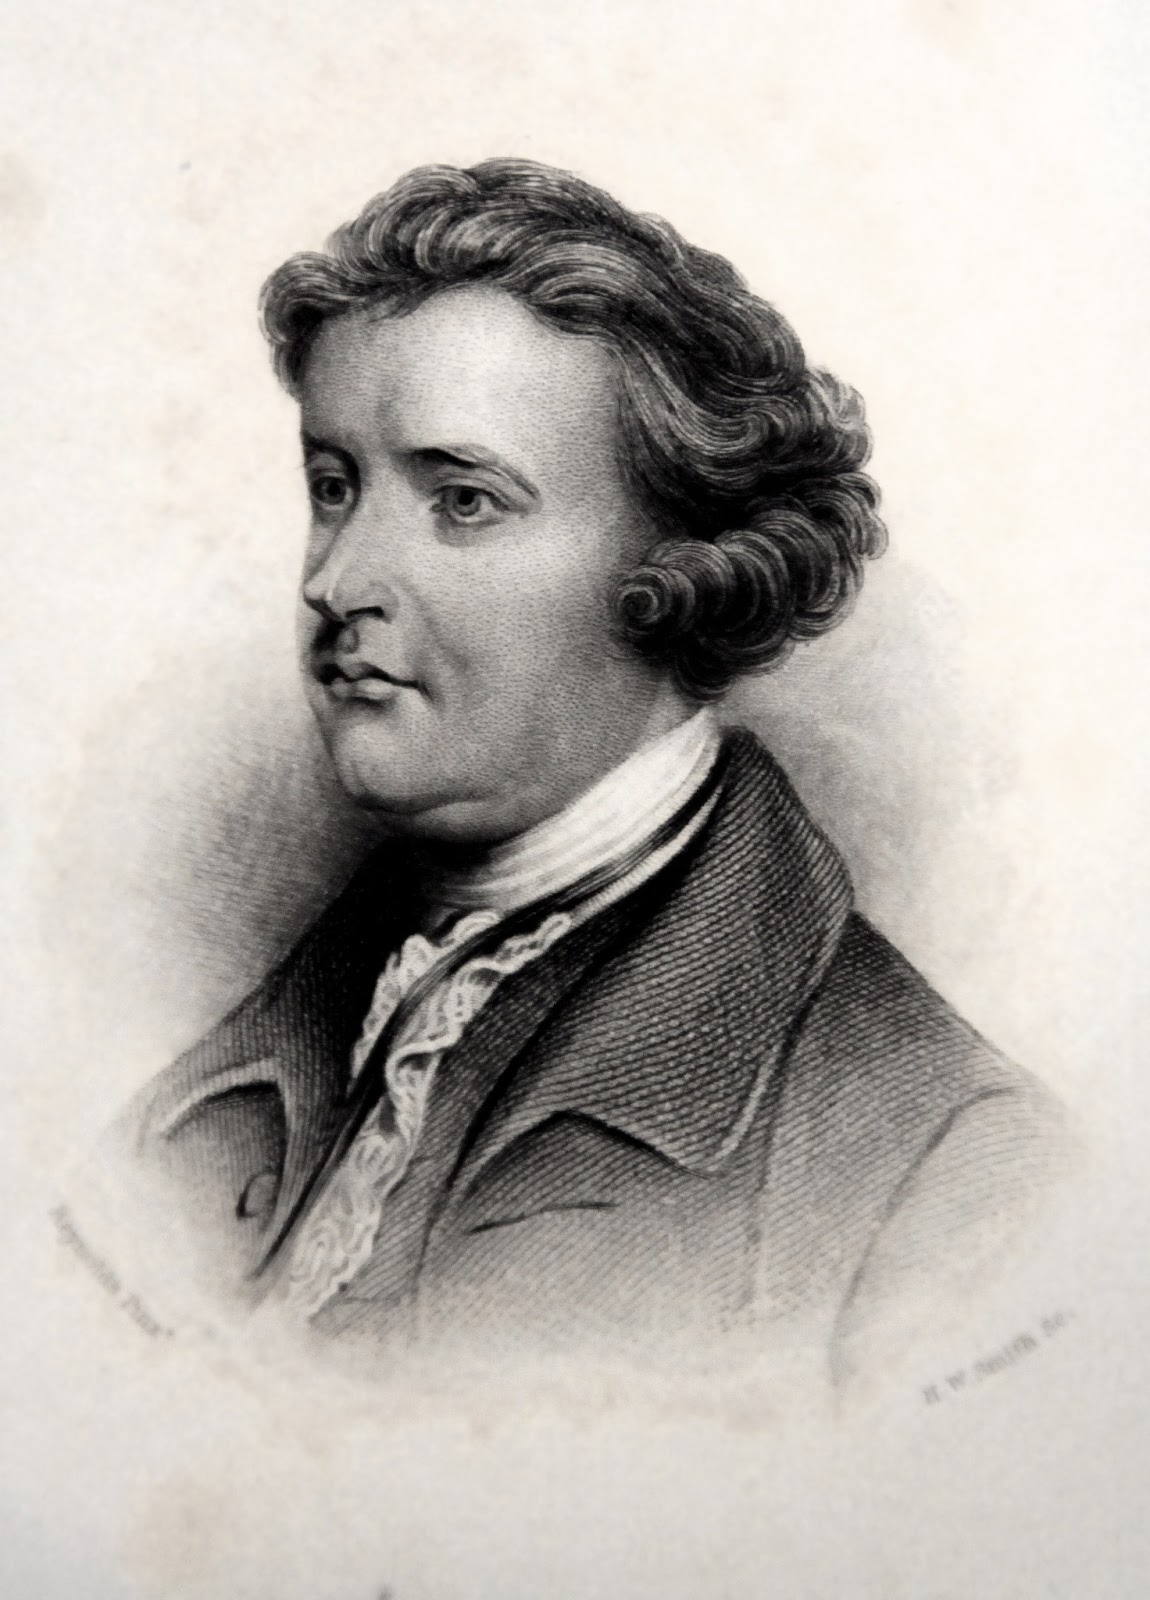
\includegraphics[width=50mm]{images/burke.jpg}
       \caption{バーク}
     \end{figure}



\subsection{}




我々が形而上学的な詭弁の迷路へ取り込まれることがない限り、確定した規則と臨機応変の方策との、つまり我が国の統治における継承なる世襲原理の神聖さと、極端な非常事態の際のその適用の変更に関する権限との両立は決して不可能ではない。あのような緊急事態に際してさえも(名誉革命におけるそれの行使で我々の権利の範囲を推し測るならば)、変更は、単に欠陥ある部分だけに、つまりこの止むをえない逸脱を生み出した部門に限定さるべきであって、この場合でさえ、それは決して市民的政治的な全機構の解体を通じて、社会の第一要素から新しい市民秩序を作り出すことがないように遂行さるべきである。

何らかの変更の手段を欠く国家は、自己の保存のための手段を持たない。かかる手段がなければ、それは自分が最も入念に保存を念願する、憲法の肝心要の部分を喪失する危険をさえ惹き起すだろう。この保存と補正なる原理は、イギリスで国王が不在であった王政復古と名誉革命という二つの重大な危局に際して、強力に機能した。この二つの時期に国民は、古来の建造物を統合する絆を喪失していたが、全構築物を解体はしなかった。逆に彼らは、この両方の場合、損傷を受けない個所を通じて古い憲法の欠陥部門を再生させた。彼らは、これら古い部分を全く旧来の姿に残したままで、再生された部分をこれに適応させた。彼らは、自分たちの旧来の組織の形に編成された古代の有機的な身分制議会によって行動し、決してばらばらに解体した民衆の組織的な分子群として行動しなかった。〔……〕(上・44-45)

\subsection{}




見られるように、マグナ・カルタから権利宣言に至るまで一貫して我が憲法の政策は、祖先から我々に伝えられ、今後は我々の子孫へと伝承さるべき限嗣財産として、つまり、この王国の民衆に特別に帰属して、それ以外の如何なる一般的ないし先行的な権利とは関連しない資産として我々の自由を要求し行使することであったことが判明する。この手法によって我が国の憲法は、諸部門のかくも無限な多様性の中で統一を保持している。我々は相続さるべき王冠、相続さるべき貴族制度、そして長い先祖の家系から権限と市民権と各種の自由を相続した下院議員と国民を有している。

私はこの方策が、深遠な反省の結果、敢えて言うならば反省抜きで反省を越えた叡智に他ならぬ、自然に追随した幸福な結果のように思われる。概して革新の精神は、利己的な性情と狭隘な視野の結果である。自分の先祖を振り返って見ようとしない徒輩は、決して自分の後裔にも目を向けないだろう。さらにイギリス国民は、相続の観点が保存と継承なる二つの確実な原理を我々に与える半面で、決して改良の精神を排除しないことを知っている。それは自由な獲得を実現しながら、獲得された財産を保全する。この種の格律にもとづく手続で国家が獲得する利得は、すべて一種の継承不動産設定の形で厳重に収蔵されて、一種の死手譲渡として永久に捕捉される。我々は自然の範例に依拠して機能するこの立憲政策によって、我々の統治と特権を、我々が自らの生命財産を享受した上で引き渡すのと同じ仕方で継承し保存して引き渡す。政策にもとづく諸制度、運勢にもとづく恩恵、天与の才能もまた、同じ経路と順路を経て我々へ、そして我々から伝えられる。

我々の政治体制は、世界全体の秩序に、つまり一過性の諸部分から成る恒久的な総体に当てがわれる存在様式に厳正に対応した均斉ある姿に置かれ、その結果、ここでは人類全体の偉大な神秘的協合体を統合する畏れ多い叡知の配剤によって、全体が或る特定にまるまる老年もしくは壮年、あるいは幼年ではありえず、不変な恒常性の条件下で一様に衰微、消滅、再生、前進なる多種多彩な過程を通じてそれは豊かな様相を呈しつつ運行する。我々がこのように国家の運営においても自然の方法を保持することで、改良された部分は一途に新規でもなく、我々が保存するものは全体がまるまる時代後れではなくなる。

我々は、この流儀とこの原理にもとづいて我らの先祖に追随することで、好古家の迷信ならぬ哲学的な類比の精神によって導かれる。この相続制度の選択によって、我々は、国家の枠組に血縁関係の心象を与えてきた。つまり我々は、我が国の憲法を我らの最愛の家族的紐帯に結びつけ、自国の基本的な法規を我らの家庭的な情愛の奥底へ組み入れることで、我々の国家、炉端、我々の墳墓と祭壇を不可分な互いに反映し合うこれらの各種の慈愛の温情で哺み、その全体を保全する訳である。

我々は人為的な制度においても、同様な自然への対応なる計画に準拠することで、自然の過つことのない強力な衝動の助けを動員して我々の理性の脆弱で誤りがちな工夫を補強することで、これ以外にも自分らの自由を相続の観点から眺めることの少なからぬ利益を引き出してきた。ややもすると放埓な行き過ぎに走りかねない自由の精神は、列聖された我々の先祖の眼前に常に自分がいるように考えることで、厳粛な畏敬の念に和らげられる。自由な継承なる観念は、我々の胸中に一種生まれつきの習慣的な威厳の念を鼓吹することで、何らかの栄誉の最初の獲得者には不可避的に随伴して品位を貶める、あの成り上がりの傲慢さを防止する。(上・66-67)

\subsection{}



確かに、国家の財産と並んで国家の有する才能を代表しないものは、その国家の適切かつ充全な代表制度ではありえない。だが、才能が活動的積極的な原理であるに反して、財産は不活発で愚鈍そして臆病である故に、財産は代表制の中であらゆる釣合を越えた圧倒的な比重を有しない限り、才能による侵害から安泰ではありえない。それはまた蓄積された巨大な集塊の形で代表されねばならず、さもないと正しい保護策にはならない。財産は、その取得と保持の結合した原理から、当然ながら不平等を特徴的な本質とする。それ故、羨望を招き強欲心を挑発する巨大財産は、危険の可能性から護られねばならず、これはその状態にあって初めて、あらゆる階梯の一層零細な財産にとっても自然な堡塁たりうる。同じ量の私有財産でも、事物の自然な進行によって多数の人間に分割される場合には、同じ機能を発揮できない。財産の分散に応じて、それの防御力は弱体化する。この分散の中の各人の持分は、その熾烈な貪欲心から、彼自身が他人の集積物の蕩尽を通じて当てにしたものよりは小さくなる。少数者の富の掠奪は、実際に多数者への配分に際しては限りなく零細な分け前しか生み出さないが、多数者はこの点の計算能力を持たないし、彼らを掠奪へ導く徒輩は、決してこの種の配分を意図しない。

自分の財産を末代まで家計に伝えるという我々の権限は、財産に付随する最も貴重で興味深い属性の一つであって、社会そのものの永続に最も有力な効果を発揮する。それは、我々の弱さを我々の美徳のために役立てる。それは、強欲心にすら慈愛の心を接木する。家計の財産とその世襲的保有に随伴する栄誉の持主は、(これに最も切実な関心を寄せる者として)この伝達の自然な保証人である。我が国の上院はこの原理にもとづいて作られ、丸々世襲的財産と世襲的な栄誉から構成されている。〔……〕

二千四百万人は二十万人よりも優位を占めるべきだ、との声がある。一国の憲法が算術の問題である限り、確かにその通りである。この種の言説は街灯柱を介添人とする限りは多少とも通用しようが、冷静な推論ができる人間には馬鹿げて映る。多数者の意思と彼らの利益は極めてしばしば喰い違うはずであり、彼らが悪しき選択を行なう場合にはその差異が甚だしくなる。五百人の田舎代言人や無名な司祭たちの統治は、よしんば彼らが四千八百万人から選ばれたところで、二千四百万人の利益には役立たないし、それが、権力獲得の意図で自己への信託を裏切った一握りの貴族連中に指導されようとも、事態は同様である。

貴国民は、今日すべての物事で自然の大道を踏み外したように思われる。フランスの財産はフランスを統治していない。私有財産はもちろん破壊されて、理性的な自由は存在の影すら見当たらない。帰国が当面実現したものは、紙幣流通と相場師の憲法だけである。そして今後、本当に貴下は、合計八十三の独立自治体による共和体制へ編成されたフランスの領土が(これらを構成する個々の部分については言わずもがな)、一つの団体として統治され、一つの精神の衝動で運営されうるなどと、本気で考えているのか?(上・95-98)

\subsection{}



統治機関は元来、それからは全く独立して、格段に明晰で格段に抽象的な完成の姿で存在する如き自然的権利のために形成されるものでは決してない。そもそも、この種の抽象的な完全さは、それの実際的な欠陥となる。彼らは万物への権利を有することで、万物を喪失する。統治は、人間の諸々の必要を実現するための、人間的叡知の考案である。人間は、この種の必要がこの叡知によって実現されることへの権利を有する。この種の必要の一つとして、文明社会内での人間の情念への充分な抑制の必要性が挙げられよう。社会は、個々人の情念の制御にとどまらず、人々の意向が単に個人としてばかりでなく、集合や集団としても頻繁に抑止され、彼らの意思が管理され、情熱が抑止されるように要請する。これは、当事者以外の者の権能によってのみ果たされる故に、この機能の発揮に際しては、決して本来これが抑制し圧伏する役目を持つべき当事者の意思ないし情熱に従ってはならない。この意味において、人間へのこの種の抑制は、彼らの自由に少しも劣らず、彼らの権利に数えられるべきである。だが、自由や抑制は時代や状況によってその様態が千差万別である以上、それらを何らかの抽象的規則にもとづいて決定することは不可能であり、この種の原理にもとづく議論以上に馬鹿げたものはない。

ある種の人為的実定的な制約を容認した上で、各人が自らを統治する全能な権利から何かを除外する瞬間から、統治の組織全体は、便宜の調整の問題となる。一国家の憲法とその権限の適正な配分を、最も微妙かつ複雑な技術の事柄にする事情がこれである。この配分は、人間の本性や人間の諸々の必要への深い知識と、社会制度の仕組によって追求さるべき各種の目的遂行を、容易もしくは困難ならしめる物事の知識を前提する。(上・111-112)

\subsection{}




この開明的な御時世にあって、私は敢えて無遠慮に公言するが、我々は概して生まれつき身についたままの感情の持主であって、貴下が見て取るように、我々の偏見を捨て去るどころか逆にそれらに非常に強く愛着しており、さらに一層気恥ずかしことに、それが他ならぬ偏見なるが故に逆にそれに愛着し、しかも、それらが長続きして一層広く世に行なわれる故にこそ、一層それに強く愛着する国民である。我々は、人間がめいめい個々人の理性の私的な元手で生活し商売することを恐れる。それは、この個人的な元手が少額であり、従って、彼らとしては国民全体と過ぎし時代の共通な銀行や元手を活用する方が好都合と考えるためである。それ故、我が国の思想家の多くは、全体的な偏見の破砕とは逆に、彼らの機敏さをこれら偏見に潜む潜在的な叡知の発見に振り向ける。彼らは滅多に失敗しないし、目当てのものを首尾よく発見すると、この偏見の上衣を投げ捨てて剥き出しの理性以外の何ものも残さないのとは逆に、むしろ理性を包含した偏見の保存こそが一層賢明な方策だ、と考える。事実、理性と合さったこの偏見は、この理性を活動させる動機と、それを永続化させる愛情を哺む。偏見は、咄嗟の場合に直ちに応用が利く。それは、予め心を叡知と美徳の安全な筋道に据えることで、決断の瞬間に人間を狐疑逡巡の状態に置くことがない。偏見は人間の美徳を彼の習慣へと仕上げ、決して一連の断片的行為のままに残さない。彼の義務感は、正しい偏見によって彼の本性の一部となる。(上・160-161)

\subsection{}




確かに社会は一つの契約である。従属的で単なるその場限りの利益のための契約は、任意に解除されてもよいだろう。だが、国家は例えば胡椒やコーヒーの、キャラコや煙草の取引やその他の卑俗な用途の物品のように、細かい一時的利益のために締結されて当事者の意向一つで解約される程度の共同事業協約と考えられるべきではない。それは、別種の崇敬の念でおのずと仰ぎ見らるべきである。事実、これは一時的な壊れ易い本性の粗野な動物的存在に資するに過ぎない物事の共同事業では断じてない。それはあらゆる学問、あらゆる芸術の共同事業、すべての美徳、すべての完徳における共同事業である。この種の共同事業の目的は、数多の世代を経ても達成されないから、それは単に生きている人々の間のみならず、現に生きている者とすでに死去した者や今後生まれる者との間の共同事業となる。個々の特定国家の個々の約定は、永遠な社会の偉大な原子契約の単なる一条項に過ぎない。それらは下位の本性を高位のものと、可視の世界を不可視の世界と連結して、あらゆる物理的本性とあらゆる精神的本性をその定められた場所に配置する不可侵の誓約が裁可する、確乎たる盟約に依拠している。それ故に人々は、自己を遥かに越えた高次の義務にもとづいて、彼らの意思をこの法に従属させる責任を有し、決してその法を彼らの意思に従属させてはならない。同時にこれら普遍的な王国内の自治的な団体も、彼らの気まぐれ一つで、偶然的な改善の思惑にもとづいて、任意にその従属的共同体の紐帯を残らずずたずたに切断して原始的要素の非社会的で粗野な個々ばらばらの混沌へと解消する真似は、道義的に許されない。無秩序への復帰を辛うじて正当化しうるのは、選択されるのでなく選択する第一の至高な止むなき必然性、如何なる考慮をも超越して一切の論議を許さず、何一つ証拠を要求しない非常事態だけである。この最終的な必要性は、決して規則への例外ではない。何故ならば、この止むをえない必然性そのものが、合意と強制の区別なく人間が服従せねばならぬ、事物のあの道徳的物理的な配置の一部を形成するからである。もしもこれと逆に、必要性への単なる服従に他ならないものが選択の対象にされるならば、法は破壊されて自然な人情は無視され、その結果これらの叛乱分子はこの理性と秩序、平和と美徳、そして稔りある悔悟の世界から狂気や不和と悪徳、そして詮ない悲嘆という対照的な世界へと法外化され、追放され、配流される。(上・177-179)

\vspace{2zw}

\section{推薦図書}


\begin{itemize}
\item 阿川尚之 (2013) 『憲法で読むアメリカ史』、ちくま学芸文庫。はじめての成文憲法をもった国アメリカで、奴隷制度や言論の自由、その他憲法をめぐってどんな戦いがおこなわれたか、現代に至るまでおもしろく読める。(江)
\item 河野健二(1959)『フランス革命小史』岩波書店。新書の中の古典。古本屋に行こう。(渡)
\item 池田理代子『ベルサイユのばら』、集英社。名作少女マンガなので必ず読みましょう。いろんな版がある。(江)
\item C. B. マクファースン、谷川昌幸訳(1988)『バーク――資本主義と保守主義』お茶の水書房。バークについての数少ない概説書。活動の多面性と思想の変遷がよくわかる。(渡)

\end{itemize}

%%% Local Variables:
%%% mode: japanese-latex
%%% TeX-master: "main_gendai"
%%% coding: utf-8
%%% End:
